\documentclass[
    xelatex,
    chapter-numbering,
    % big,
]{G7-32-2017}

\usepackage{lipsum}

% \usepackage{amsthm,amsfonts,amsmath,amssymb,amscd}
% % \usepackage[T2A]{fontenc}
% % \usepackage[utf8]{inputenc}
% % \usepackage[english,russian]{babel}
% \usepackage{float}
\usepackage{graphicx}
% % \usepackage{cmap}
% \usepackage{color}


% \usepackage[all,cmtip]{xy}
\graphicspath{ {./pictures/} }

% % \usepackage{subcaption}
% \usepackage{cite}

% % \usepackage{dsfont}
% % \usepackage{mathrsfs}

% \TableInChaper
% \PicInChaper
% \setlength\GostItemGap{2mm}


% \NirOrgLongName{\MakeUppercase{Название организации}}

% \NirBoss{Должность руководителя организации}{ФИО} %% Заказчик, утверждающий НИР
% \NirManager{Должность руководителя НИР}{ФИО}

% \NirTown{[ГОРОД],}
% \NirYear{[ГОД ОТЧЕТА]}

% \NirUdk{УДК \No }
% \NirGosNo{Регистрационный \No }

% \NirStage{
% }{[ТИП ОТЧЕТА], за [ГОД] г.}{
% }

% \bibliographystyle{unsrt}

% \newtheorem{theorem}{Теорема}[chapter]
\newtheorem*{theorem*}{Теорема}
\newtheorem*{lemma*}{Лемма}
\newtheorem{property}{Свойство}
\newtheorem{lemma}{Лемма}[chapter]
\newtheorem{statement}{Утверждение}[chapter]
\newtheorem{definition}{Определение}[chapter]
\newtheorem{example}{Пример}[chapter]
\newtheorem{corollary}{Следствие}[chapter]
\newtheorem*{corollary*}{Следствие}
\newtheorem{remark}{Замечание}[chapter]
\newtheorem*{remark*}{Замечание}
\newtheorem{hypothesis}{Гипотеза}[chapter]

\newtheorem{cond}{Условие}
\newtheorem{theoremA}{Теорема}
\newtheorem{lemmaA}{Лемма}[section]
\newtheorem{state}{Предложение}
\newtheorem{proposition}{Предложение}
\renewcommand{\thetheoremA}{\Alph{theoremA}}
\renewcommand{\thelemmaA}{\thesection.\Alph{lemmaA}}
\newcommand{\No}{\textnumero}

\newcommand{\norm}[1]{\|#1\|_{p(\cdot),w}}
\newcommand{\ip}[2]{\langle #1, #2 \rangle}

\DeclareMathOperator*{\esssup}{ess\,sup}
\DeclareMathOperator*{\essinf}{ess\,inf}

\numberwithin{equation}{chapter} %
\renewcommand{\theequation}{\thechapter.\arabic{equation}}

\newenvironment{description}{}{}

\newcommand{\ifNotEmpty}[2] {
    \ifx&#1& \empty \else #2 \fi
}

\newcommand{\row}[3][]{
    \small{#2}&
    \centering{\rule[-2mm]{5cm}{0.2mm}} \newline \centering \footnotesize{{подпись, дата}} &
    #3 \newline \small{{\ifNotEmpty{#1}{(#1)}}} \\ & & \\
}

% \usepackage[shortlabels]{enumitem}


% %%%%%%%<------------- НАЧАЛО ДОКУМЕНТА
\begin{document}

% Руководитель НИР
\HeadOfResearch[№ раздела]{должность}{И.О.~Фамилия}

% Титульная страница
\TitlePage{content/titlePage}

\frontmatter

\Executors{content/executors.tex}
\Referat{content/referat.tex}
\tableofcontents
\Defines{content/defines.tex}
\Abbreviations{content/abbreviations.tex}
\Introduction{content/introduction.tex}

\mainmatter

\chapter{Chapter}

\section{Section}

\subsection{Subsection}

\lipsum

Ссылка на рисунок \ref{ex:fig:1}.
\begin{figure}[h]
    \centering
    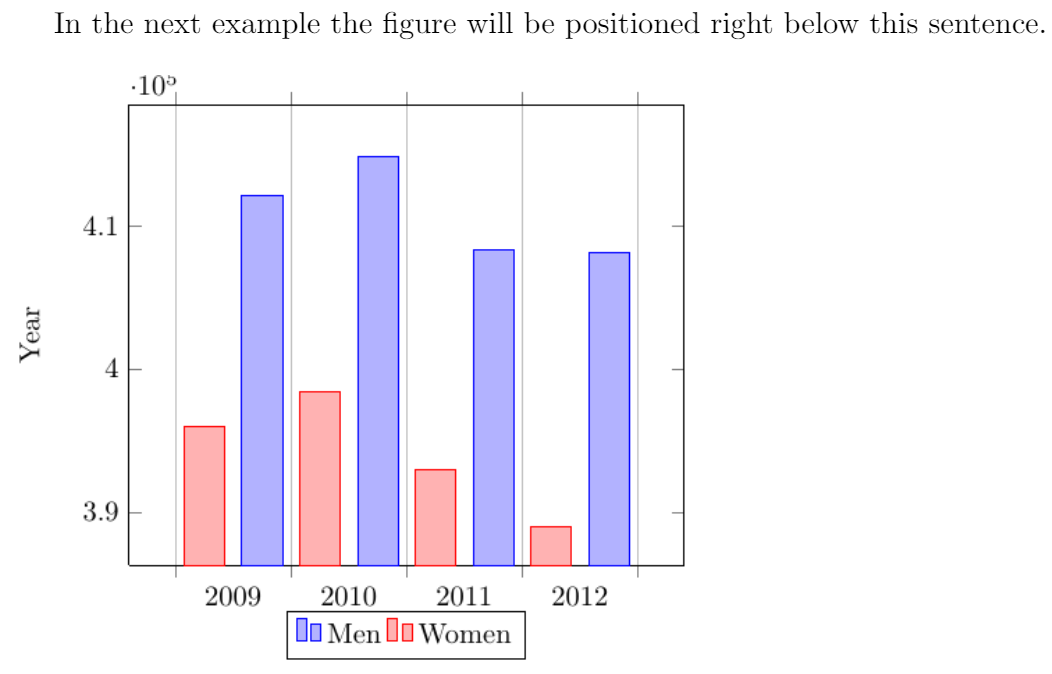
\includegraphics[width=8cm]{[NAME]/Plot}
    \caption{\lipsum[6][4-5]}
    \label{ex:fig:1}
\end{figure}

Ссылка на таблицу \ref{ex:tb:1}.
\begin{table}[h]
    \centering
    \caption{\lipsum[3][3-5]}
    \label{ex:tb:1}
    \begin{tabular}{| c | c | c | c |}
        \hline
        Col1 & Col2 & Col2 & Col3 \\
        \hline
        1 & 6 & 87837 & 787 \\
        \hline 
        2 & 7 & 78 & 5415 \\
        \hline
        3 & 545 & 778 & 7507 \\
        \hline
        4 & 545 & 18744 & 7560 \\
        \hline
        5 & 88 & 788 & 6344 \\
        \hline
    \end{tabular}
\end{table}

\lipsum[1][1]
\begin{enumerate}
    \item \lipsum[1][1-2]
    \item \lipsum[1][3-4]
    \item \lipsum[1][5-6]
    \item \lipsum[1][1-2]
    \item \lipsum[1][3-4]
    \item \lipsum[1][5-6]
    \item \lipsum[1][1-2]
    \item \lipsum[1][3-4]
    \item \lipsum[1][5-6]
    \item \lipsum[1][1-2]
    \item \lipsum[1][3-4]
    \item \lipsum[1][5-6]
    \item \lipsum[1][1-2]
    \item \lipsum[1][3-4]
    \item \lipsum[1][5-6]
    \begin{enumerate}
        \item \lipsum[2][1-3]
        \item \lipsum[2][2]
        \item \lipsum[2][3]
    \end{enumerate}
\end{enumerate}
\begin{itemize}
    \item \lipsum[1][1-2]
    \item \lipsum[1][3-4]
    \item \lipsum[1][5-6]
    \begin{itemize}
        \item \lipsum[2][1-3]
        \item \lipsum[2][2]
        \item \lipsum[2][3]
    \end{itemize}
\end{itemize}

Пример текста на русском языке с ссылкой на формулу \eqref{ex:eq:1}.
\begin{equation}
    \label{ex:eq:1}
    e = mC^2
\end{equation}

\backmatter

\Conclusion{content/conclusion.tex}

\begin{thebibliography}{111}

  % Ниже указаны примеры форматирования литературы

  \bibitem{mmg-MarcellanXu2015}
  Marcellán F., Xu Y. On Sobolev orthogonal polynomials // Expositiones Math. --- 2015. --- Vol 33. P. 308---352.

  \bibitem{mmg-mmg-walsh-Shii-UMN}
  Шарапудинов И.И. Ортогональные по Соболеву системы функций и некоторые их приложения // УМН. --- 2019. --- Т. 74, \No 4(448). --- С. 87---164.

  \bibitem{ark-bib-2}
  Стечкин С.Б., Субботин Ю.Н.
  Сплайны в вычислительной математике.
  --- М.: Наука,
  1976. --- 248~с.

  \bibitem{ark-bib-3}
  Завьялов Ю.С., Квасов Б.И., Мирошниченко В.Л.
  Методы сплайн-функций.
  --- М.: Наука,
  1980.
  --- 352 c.

\end{thebibliography} 

\appendix

\chapter{Пример приложения}

\lipsum[3-5]

Reference to appendix formula \eqref{ex:eq:a:1}.
\begin{equation}
    \label{ex:eq:a:1}
    e = mC^2
\end{equation}

\chapter{Еще один пример приложения}

\lipsum[1-2]

% % \usefont{T2A}{ftm}{m}{} %%% Использование шрифтов Т2 для возможности скопировать текст из PDF-файлов.

% \frontmatter %%% <-- это выключает нумерацию ВСЕГО; здесь начинаются ненумерованные главы типа Исполнители, Обозначения и прочее

% \NirTitle{\begin{center}
{\large
[НАЗВАНИЕ ТЕМЫ]
}
\\[12pt]
\end{center}
}

% \Executors %% Список исполнителей здесь
% % %%% это рисует линию размера 3мм и толщиной 0.1 пункт
% \begin{longtable}{p{0.35\linewidth} p{0.305\linewidth} p{0.33\linewidth}}
    
    Руководитель НИР, & & \\
    \row[№ РАЗДЕЛА]{[ДОЛЖНОСТЬ]}{[И.О. ФАМИЛИЯ]}

    Отв. исполнители: & & \\
    \row[№ РАЗДЕЛА]{[ДОЛЖНОСТЬ]}{[И.О. ФАМИЛИЯ]}
    \row[№ РАЗДЕЛА]{[ДОЛЖНОСТЬ]}{[И.О. ФАМИЛИЯ]}
    \row[№ РАЗДЕЛА]{[ДОЛЖНОСТЬ]}{[И.О. ФАМИЛИЯ]}

    Исполнители: & & \\
    \row[№ РАЗДЕЛА]{[ДОЛЖНОСТЬ]}{[И.О. ФАМИЛИЯ]}
    \row[№ РАЗДЕЛА]{[ДОЛЖНОСТЬ]}{[И.О. ФАМИЛИЯ]}
    \row[№ РАЗДЕЛА]{[ДОЛЖНОСТЬ]}{[И.О. ФАМИЛИЯ]}

    \row[]{Нормоконтроль}{[ФИО]}

\end{longtable}


% % Настройки реферата
% [Количество книг]
% \TotalBooks{0}
% [Количество рисунков]
% \TotalFigures{0}
% [Количество таблиц]
% \TotalTables{0}
% [Количество использованных источников]
% \TotalBibItems{0}
% [Количество приложения]
% \TotalAppendixes{0}

% Ключевые слова
\KeyWords{Ключевые слова}

% Оптимальный объем (~850 печатных знаков)
[Реферат отчёта, не более 1 страницы]

% \setcounter{tocdepth}{2} %hide subsections

% \tableofcontents

% %\NormRefs % Нормативные ссылки
% %\Defines % Необходимые определения

% \Abbreviations %% Список обозначений и сокращений в тексте

% [В этом файле должно быть записано общее для отдела введение]

% \mainmatter %% это включает нумерацию глав и секций в документе ниже

% \chapter{Тема основной части отчета сотрудника}

[Здесь должны содержаться основные результаты отчета с учетом введения и заключения]

% \backmatter %% Здесь заканчивается нумерованная часть документа и начинаются заключение и ссылки

% \Conclusion

[Общее заключение для всей темы отчета]% заключение к отчёту
% \begin{thebibliography}{111}

  % Ниже указаны примеры форматирования литературы

  \bibitem{mmg-MarcellanXu2015}
  Marcellán F., Xu Y. On Sobolev orthogonal polynomials // Expositiones Math. --- 2015. --- Vol 33. P. 308---352.

  \bibitem{mmg-mmg-walsh-Shii-UMN}
  Шарапудинов И.И. Ортогональные по Соболеву системы функций и некоторые их приложения // УМН. --- 2019. --- Т. 74, \No 4(448). --- С. 87---164.

  \bibitem{ark-bib-2}
  Стечкин С.Б., Субботин Ю.Н.
  Сплайны в вычислительной математике.
  --- М.: Наука,
  1976. --- 248~с.

  \bibitem{ark-bib-3}
  Завьялов Ю.С., Квасов Б.И., Мирошниченко В.Л.
  Методы сплайн-функций.
  --- М.: Наука,
  1980.
  --- 352 c.

\end{thebibliography} 
% \chapter{Cписок работ, опубликованных \texorpdfstring{\\ }{} по теме НИР в [ГОД] г.}

% Ниже представлены примеры опубликованных работ

\section*{Список опубликованных научных статей}

\begin{enumerate}
    \item
    {[Авторы]}
    [Название статьи]
    //
    [Название журнала].
    --- [год выпуска].
    --- Т. [номер тома], вып [номер выпуска].
    --- С.~[страница начала статьи]---[страница конца статьи].

    \item
    \foreignlanguage{english}{%
        Sultanakhmedov, M.S.
        Approximation of Functions by Discrete Fourier Sums in Polynomials Orthogonal on a Nonuniform Grid with Jacobi Weight.
        //
        Math Notes. 
        --- 2021.
        --- Vol. 110.
        --- P.~418---431.
    }%

    \item
    \foreignlanguage{english}{%
        Gadzhimirzaev, R.M., Shakh-Emirov, T.N.
        Approximation Properties of the Vallée-Pous\-sin Means of Partial Sums of a Special Series in Laguerre Polynomials.
        //
        Math Notes. 
        --- 2021.
        --- Vol. 110.
        --- P.~475---488.
    }%

\end{enumerate}

\section*{Список зарегистрированных программ для ЭВМ}

\begin{enumerate}

    \item
    {[Авторы]} Свидетельство №[номер свидетельства] о государственной регистрации программы для ЭВМ <<[название программы]>>. Заявка №[номер заявки], дата поступления [дата поступления заявки]. Дата государственной регистрации в Реестре программ для ЭВМ [дата гос. регистрации]. Правообладатель: ДФИЦ РАН.

    \item
    {[Авторы]} Свидетельство №[номер свидетельства] о государственной регистрации программы для ЭВМ <<[название программы]>>. Заявка №[номер заявки], дата поступления [дата поступления заявки]. Дата государственной регистрации в Реестре программ для ЭВМ [дата гос. регистрации]. Правообладатель: ДФИЦ РАН.

\end{enumerate}


\end{document}
